\documentclass[12pt,a4paper]{article}
\usepackage[utf8]{inputenc}
\usepackage[english]{babel}
\usepackage[T1]{fontenc}
\usepackage{amsmath}
\usepackage{amsfonts}
\usepackage{amssymb}
\usepackage{graphicx}
\usepackage[final,pdftex, colorlinks=false]{hyperref}
\usepackage{xcolor}
%\usepackage{comment}
%\usepackage{floatrow}
%\usepackage{multirow}
%\usepackage{algorithm}
%\usepackage{algorithmicx}
%\usepackage{algpseudocode}
%\usepackage{titletoc}
%\usepackage{pdfpages}
%\usepackage{hhline}
%\usepackage{makecell}

\usepackage{listings}			%vkladani kodu
\lstset{basicstyle=\ttfamily,
  showstringspaces=false,
  commentstyle=\color{red},
  keywordstyle=\color{blue},
  breaklines=true,
  frame=lines,
}

%okraje
\usepackage[
left=35mm,
right=25mm,
top=40mm,
bottom=35mm]
{geometry}

\author{David Těthal}

%%%%%%%%%%Prikazy%%%%%%%%%%
\renewcommand\baselinestretch{1.3}		%radkovani
\parskip=0.8ex plus 0.4ex minus 0.1 ex	%mezera mezi odstavci

\newcommand{\keywords}[2]{\noindent\textbf{#1: }#2}
\newcommand{\necislovana}[1]{%
\phantomsection
\addcontentsline{toc}{section}{#1}

%\newcommand{\exedout}{%
%  \rule{0.8\textwidth}{0.5\textwidth}%
%}


\section*{#1}
\markboth{\uppercase{#1}}{}
}
%%%%%%%%%%%%%%%%%%%%%%%%%%%%

%%%%%%%%%%Zahlavi%%%%%%%%%%%
\usepackage{fancyhdr}
\fancyhead[L]{Česte vysoké učení technické v Praze}
\setlength{\headheight}{16pt}
%%%%%%%%%%%%%%%%%%%%%%%%%%%%

\begin{document}
\pagestyle{empty}

%titulni strana
\newpage
\begin{center}
%napisy
\newcommand{\napisCVUT}{České vysoké učení technické v Praze}
\newcommand{\napisFS}{Fakulta Stavební}
\newcommand{\napisProgram}{Studijní program Geodézie a Kartografie}
\newcommand{\napisObor}{Obor Geomatika}
\newcommand{\napisKatedra}{Katedra Geomatiky}
\newcommand{\napisVedouci}{Vedoucí: Ing. Martin Landa, Ph.D.}
\newcommand{\napisAutor}{Bc. David Těthal}
\newcommand{\napisDatum}{Praha 2018}
\newcommand{\napisNazevI}{Rozšíření platformy Gisquick o podporu časoprostorových dat}
\newcommand{\napisDiplomka}{Diplomová práce}
%
% prikazy
%\newcommand{\velka}[1]{\uppercase{#1}}
\newcommand{\velka}[1]{\textsc{#1}}
%
% 
\newif\ifpatitul
\patitultrue


{\Large\velka{\napisCVUT}}\\
{\Large\velka{\napisFS}}\\
{\Large\velka{\napisProgram}}\\
{\Large\velka{\napisObor}}
\vfill

\includegraphics[width=3cm]{./img/logo_cvut_cb} %~
\vfill
{\Large\velka{\napisDiplomka}}\\
\Large\velka{\napisNazevI}\\
\vfill
{\large%
\napisVedouci\\
\napisKatedra\\
\bigskip
\napisDatum\hfill\napisAutor}
\end{center}


%zadani prace
\newgeometry{left=1.8cm,top=2cm} 
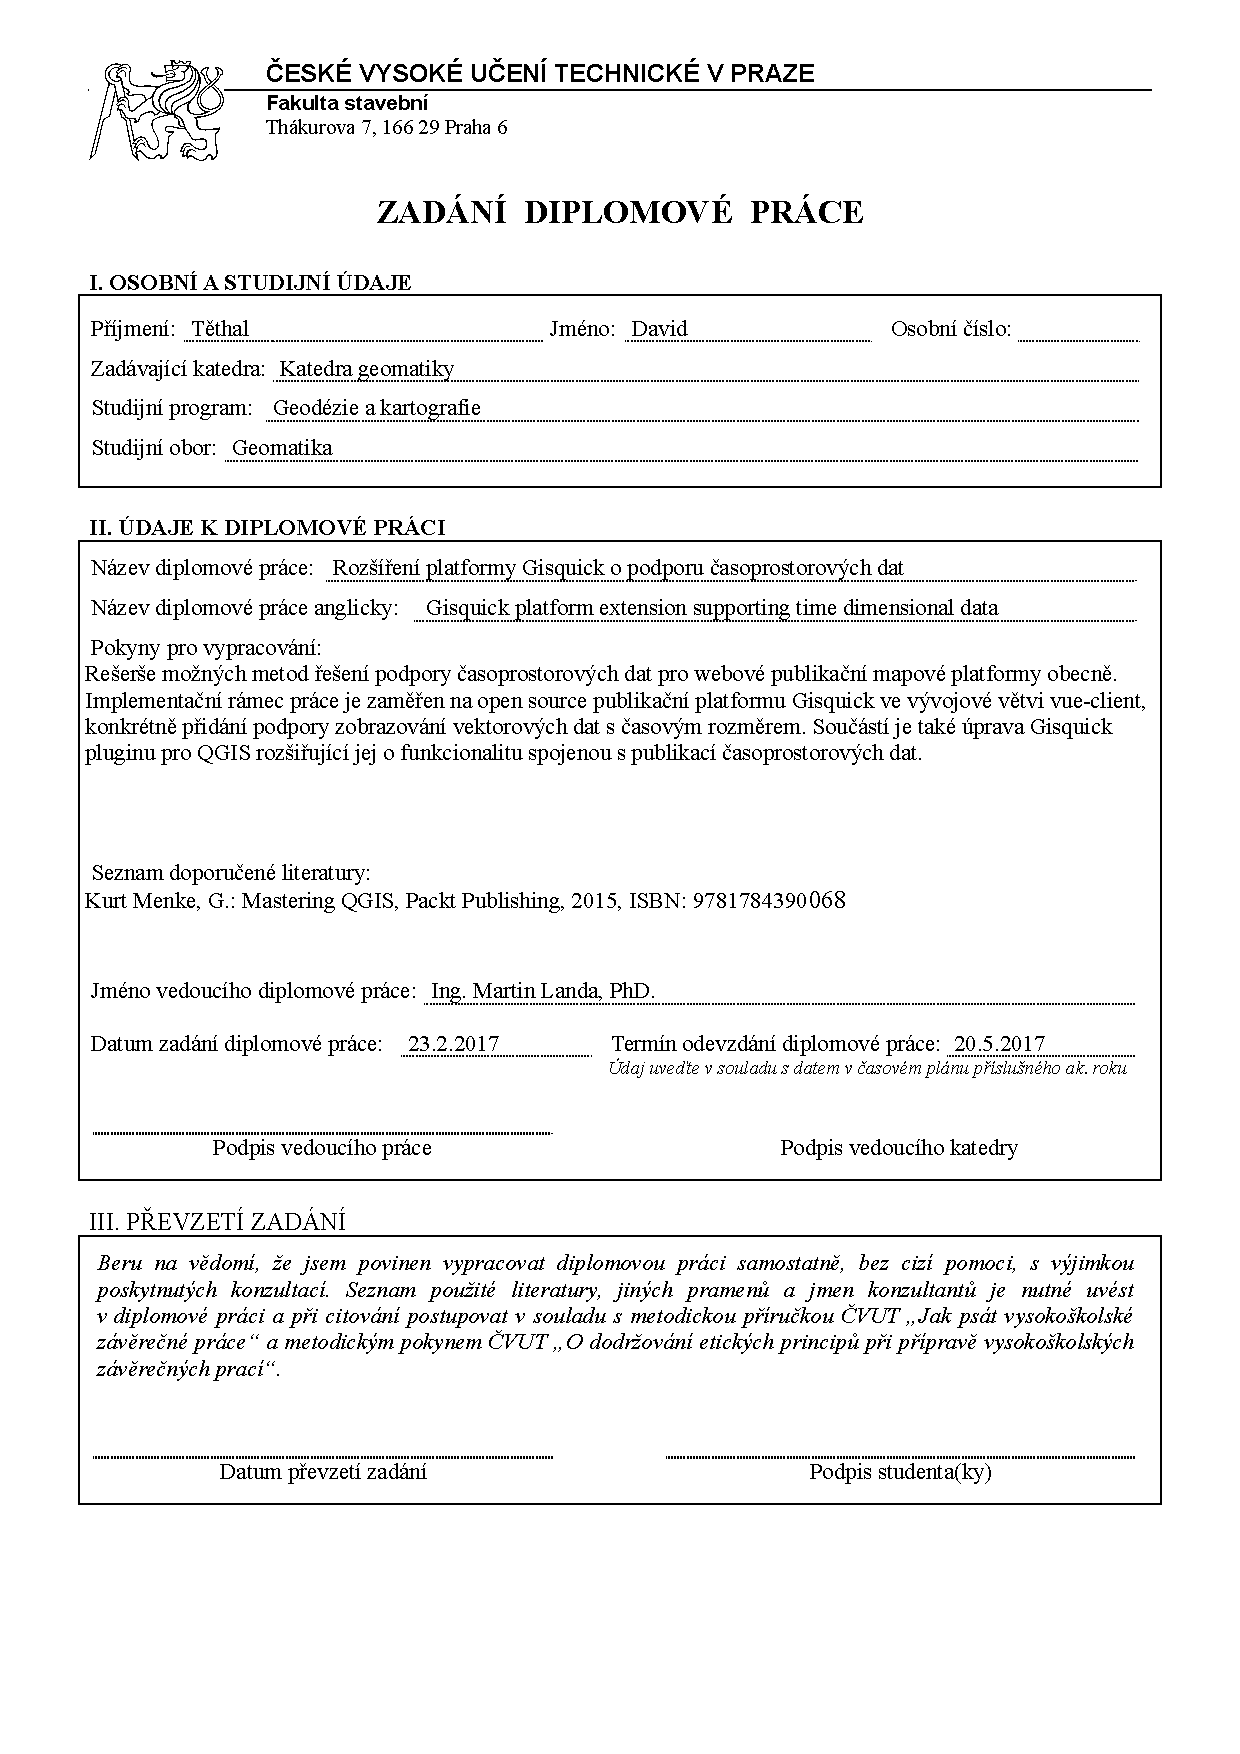
\includegraphics[scale=0.8]{../zadani/zadanidp}
\restoregeometry

%abstract CS
\newpage
\selectlanguage{english}
\begin{abstract}
\bigskip
Cílem této diplomové práce bylo navrhnutí a vytvoření nástroje pro platformu Gisquick, který umožní pracovat s časoprostorovými daty. Gisquick platforma umožňuje snadnou a rychlou publikaci projektu vytvořeného v programu QGIS. Pomoci nového nástroje bude moci uživatel snadno a rychle pracovat s vrstvy obsahující časoprostorová data, jednotlivě je filtrovat a vytvářet jednoduché animace.

V první řadě byla provedena rešerše možných obecných řešení pro webové publikační platformy. Na základě toho bylo vybráno optimální řešení, které bylo vhodně aplikované pro již stávající platformu.

Dalším krokem byla implementace nalezeného řešení na straně Gisquick klienta. Nástroj byl vyvíjen v programovacím jazyce JavaScript s použitím frameworku Vue.js, do kterého je stávající klient přepisován. 

Pro možnosti práce s časoprostorovými daty bylo dále nutné upravit zásuvný modul QGIS sloužícího k publikaci předem vytvořených projektů. Pomocí něj je možné pro jednotlivé vrstvy vybrat atribut obsahující časovou složku ve formě textového řetězce.

\bigskip
\bigskip
\keywords{Klíčová slova}
OGC WMS, časoprostorová data, QGIS, JavaScript, Python, Vue.js, plugin.
\end{abstract}

%abstract EN
\newpage
\selectlanguage{english}
\begin{abstract}
	\bigskip
	Tato diplomová práce se věnuje možnostem izolace procesů v rámci frameworku PyWPS jako jedné z implementací OGC WPS. Web Processing 
	Service je standard vydaný a dále rozšiřovaný Open Geospatial Consorciem. 
	
	První část popisuje samotný standard včetně všech základních požadavků \textit{GetCapabilities}, \textit{DescribeProcess} a \textit{Execute}.
	V závěru první části jsou zmíněny některé z implementací WPS standardu.
	
	Druhá část se zaměřuje na \textit{PyWPS}, což je implementace WPS
	standardu napsaná v programovacím jazyce Python. Čtenáři jsou
	seznámeni jak se současným stavem PyWPS, tak s projektem
	\textit{PyWPS-demo}, ukázkovou instancí PyWPS serveru, na kterém je
	postavena praktická část.  Následuje rešerše, která mapuje možné
	řešení izolace procesů, a nakonec je popsána \textit{Docker}
	technologie, která slouží pro kontejnerizaci. Tato technologie byla vybrána pro
	samotnou implementaci izolace.
	
	Poslední část se zabývá použitím Docker kontejnerů pro izolaci procesů. Detailně je vysvětleno, jak funguje \textit{Execute} operace a následně je popsána nově vytvořená třída \textit{Container} se všemi svými metodami.
	
	\bigskip
	\bigskip
	\keywords{Klíčová slova}
	OGC WPS, PyWPS, Docker kontejner, Python, izolace procesu, geoprocesing, zpracování dat.
\end{abstract}


%Prohlaseni a podekovani
\selectlanguage{english}
\newcommand{\odsaditodzhora}{\hskip1pt\vfill}
\newpage
\odsaditodzhora
\noindent {\bf Prohlášení}
Tímto prohlašuji, že diplomovou práci na uvedené téma jsem včetně výzkumu a implementace vypracoval samostatně.
Použitá literatura a podkladové materiály jsou uvedeny v seznamu zdrojů.


\begin{flushleft}
\begin{tabular}{cp{0.3\textwidth}c}
V Praze .................
& 
&
..................................
\\
&&
(podpis autora)
\end{tabular}

\end{flushleft}
\newpage

\odsaditodzhora
\noindent {\bf Poděkování}
text poděkování
\newpage
\tableofcontents

\newpage
\pagestyle{fancy}

\necislovana{Úvod}

Časoprostorová data jsou pro mnoho lidí velice obecný pojem, pod
kterým si často nedovedou nic konkrétního představit. Takto označovaná
data jsou v dnešní době již běžně používána ve velké řadě oborů od
archeologie, geodézie, geologie, stavebního inženýrství, územního
plánování až po armádní účely, zemědělství a meterologii. Nejedná se
tedy v žádném případě o specializovaný termín používaný pouze v jednom
vědním oboru.

%% ML: Na jedne strane?
Práci s časoprostorovými daty lze rozdělit na dvě skupiny. Na jedné
jsou odborníci, kteří časoprostorová data sbírají, provádějí analýzy,
vyhodnocují je pomoci specializovaných programů a vytvářejí nad nimi
tématické mapy. Na druhé straně je poté široká veřejnost, která
používá pouze finální produkt jejich práce.

V dřívější době byla možnost publikace těchto dat jen velice
omezena. To se v dnešní době s rozšířením internetu a nástupem
elektronicky publikovaných map pomoci publikačních platforem rapidně
%% ML: male p anebo do uvozovek
změnilo. Právě Publikační platformy vyplňují mezeru mezi odborníky a
širokou veřejností, kdy dávají téměř každému možnost prezentace dat v
ucelené formě.


Spojení publikační platformy a časoprostorových dat je potom dalším
krokem, který možnost prezentace dat ještě umocní. Pomocí vhodně
vytvořených nástrojů pro filtrování dat na základě jejich časové osy
se dají vytvářet simulace zobrazující průběh určitého vlivu v čase na
určitém místě. Tímto způsobem se dá například jednoduchým způsobem
simulovat vývoj požárů, migrace zvěře, nebo expanze měst. Pro
uživatele lepšího časového vjemu lze rovněž dosáhnout, vytvořením
názorné animace, kdy se zobrazovaný stav mění s předem nastaveným
časovým krokem.

Jednou z takových publikačních platforem je právě Gisquick. V tomto
případě se navíc jedná o interaktivní platformu, kde může uživatel
nejenom na data nahlížet, ale také měnit způsob jejich vizualizace. Ke
stávajícím datům se rovněž dají přidat podkladové vrstvy, které
uživateli zlepší celkový pohled na zobrazovanou situaci. Výhodou při
publikaci časoprostorových dat na platformě Gisquick je také jejich
univerzálnost. Nezáleží tedy, zdali jsou data s odstupem minut či
roků. Díky jednoduchému nastavení lze nástroj přizpůsobit téměř
jakémukoli časovému intervalu. Velká benevolence je rovněž ve vstupním
formátu časového řetězce.

\bigskip
Na platformu Gisquick resp. její rozšíření o podporu pro
časoprostorová data se zaměřuje obsah této práce. Hlavní téma je
%% ML: Nekde bys mel explicitne napsat, ze rastrova data nejsou v
%% ramci prace resena
zaměřeno na implementaci rozhraní pro podporu zobrazování vektorových
dat obsahujících časovou složku. V práci je podrobně popsán nástroj
pro práci s časoprostorovými daty, jeho jednotlivé části a jeho
implementace na platformě Gisquick.

Součástí implementace je také část zaměřena na rozšíření zásuvného
%% ML: vlozeno -> pridano?
modulu pro program QGIS. Do něj bylo vloženo nutné uživatelské
rozhraní umožňující uživateli zvolit pro jednotlivé vrstvy jejich
časový atribut tj. atribut obsahující časovou hodnotu. V této
závěrečné části je popsán samotný plugin, jeho funkce v publikaci
projektu a postup, kterým je jeho bylo uživatelské rozhraní doplněno.

%% ML: dvakrat ve vete ``platforma''
S rozšířením platformy také úzce souvisí výzkum možných metod práce s
časoprostorovými daty použitelných pro platformu Gisquick. Rešerše již
aplikovaných metod na webových mapových serverech a aplikacích je
obsažena v první části práce.
%Je zde rovněž rozebrán způsob práce s časoprostorovými daty pro webové platformy obecně a stručný popis jejich základního fungování.


%\include{appendix}

\newpage
\necislovana{Seznam zkratek}

\begin{tabular}{ll}
%\textbf{API}& Application Programming Interface\\
\end{tabular}

\newpage
\begin{thebibliography}{99}
\label{Bibliography}
%\bibitem{OGC_news}
%Mark Reichardt \textit{OGC Newsletter - October 2004, OGC document number 04-043} [online].
%%URL: \textless\url{http://www.opengeospatial.org/pressroom/newsletters/200410}\textgreater

\end{thebibliography}


\end{document}
